\section{Runtime View}
\subsection{Runtime Overview}

\begin{figure}[ht]
  \centering
  \includegraphics[width=\textwidth]{resources/03-runtime-view/pdf/cloud-ressources.pdf}
  \caption{Übersicht über die Cloud Ressourcen}
  \label{fig:cloud-ressources}
\end{figure}

\begin{figure}[ht]
  \centering
  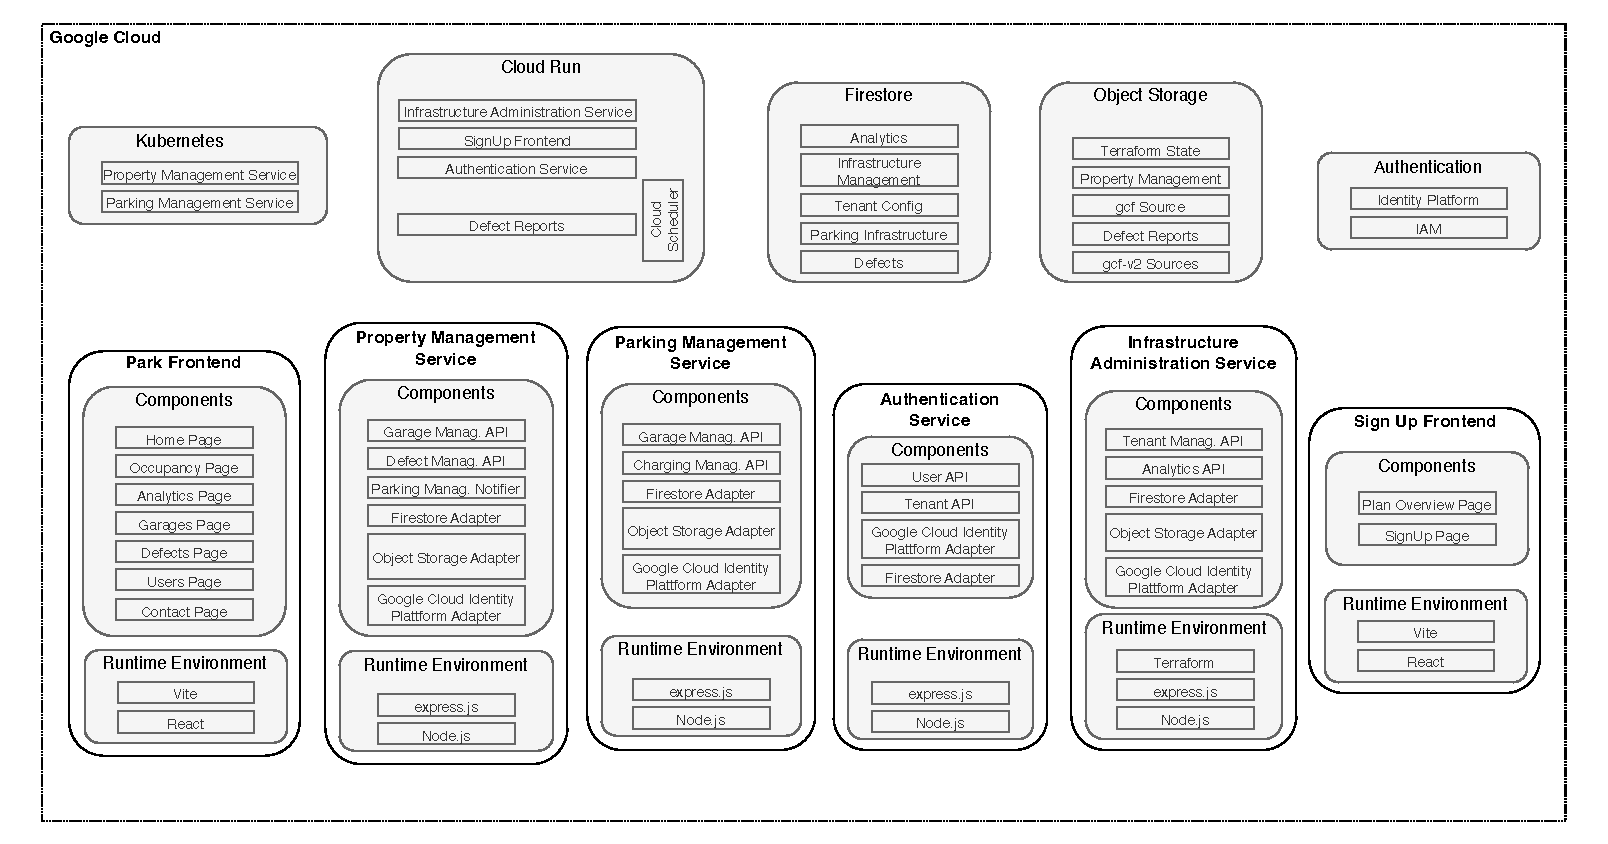
\includegraphics[width=\textwidth]{resources/03-runtime-view/pdf/architecture.pdf}
  \caption{Alle Mircoservices}
  \label{fig:system-architecture}
\end{figure}

In Abbildung \ref{fig:cloud-ressources} ist die Übersicht über die Cloud Ressourcen dargestellt. 
Die Cloud Ressourcen sind in zwei Gruppen unterteilt:
\paragraph{}

\begin{figure}[ht]
  \centering
  \includegraphics[width=\textwidth]{resources/03-runtime-view/pdf/authentication-sequence.pdf}
  \caption{Ablauf der Tenant Typ abhängigen Authentifizierung}
  \label{fig:authentication-sequence}
\end{figure}


\begin{figure}[ht]
  \centering
  \includegraphics[width=0.95\textwidth]{resources/03-runtime-view/pdf/components-frontend-park.pdf}
  \caption{Alle verwendeten Komponenten, wenn ein Client mit dem Park Frontend interagiert, mit Berücksichtigung von Multitenancy}
  \label{fig:03-components-park-frontend}
\end{figure}

\begin{figure}[ht]
  \centering
  \includegraphics[width=\textwidth]{resources/03-runtime-view/pdf/components-frontend-signup.pdf}
  \caption{Alle verwendeten Komponenten, wenn ein Client mit dem Signup Frontend interagiert}
  \label{fig:03-components-signup-frontend}
\end{figure}

\subsection{Mircoservices}
\subsection{Data Stores}